\section{氢气的制取和性质}\label{sec:xssy-sy4}

\begin{shiyanmudi}
    1. 学会实验室制取氢气和检验氢气纯度的方法; 2. 试验氢气的重要化学性质。
\end{shiyanmudi}


\begin{shiyanyongpin}
    试管、烧杯、酒精灯、铁架台(带铁夹)、单孔橡皮塞、导管、橡皮管、水槽。

    锌粒、稀硫酸($1:4$)\footnote{稀硫酸 ($1:4$)指的是 1 体积浓酸跟 4 体积蒸馏水混和而配成的溶液。}、氧化铜。
\end{shiyanyongpin}


\begin{shiyanbuzhou}
    1. 制取氢气和检验氢气的纯度

    (1) 照图 \ref{fig:xssy-19} 那样把发生氢气的装置连接好,检查这个装置的气密性。

    \begin{figure}[htbp]
        \centering
        \begin{minipage}[b]{7cm}
            \centering
            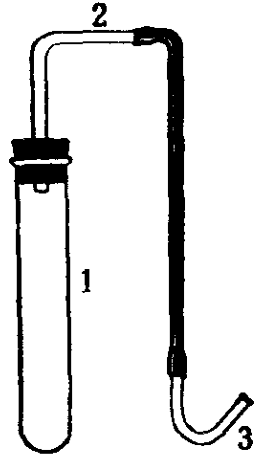
\includegraphics[width=2.8cm]{../pic/czhx1-xssy-19}
            \caption{制取氢气的简单装置}\label{fig:xssy-19}
        \end{minipage}
        \qquad
        \begin{minipage}[b]{7cm}
            \centering
            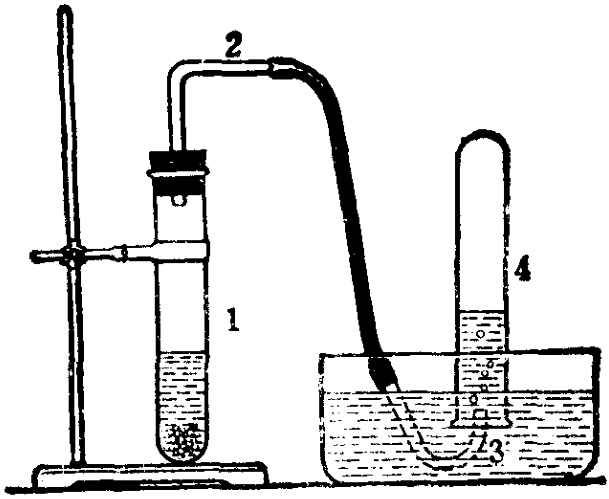
\includegraphics[width=6cm]{../pic/czhx1-xssy-20}
            \caption{制取氢气}\label{fig:xssy-20}
        \end{minipage}
    \end{figure}

    (2) 试管 1 里放入锌粒约 4 克,并注入稀硫酸(占试管 1 容积的 1/3)。
    立即用带有导管 2 的橡皮塞塞住管口,并把这个试管固定在铁架台上。

    锌粒跟稀硫酸接触后,可观察到什么现象?写出这个反应的化学方程式。

    (3) 将试管 4 装满水,用大拇指堵住管口,使管口向下,放入水中,然后照图 \ref{fig:xssy-20} 那样将导管 3 插入试管 4 里收集气体。
    当试管已集满气体时,用右手拿管底,管口朝下,一拿出水面,立即移近酒精灯火焰,点燃试管里的气体,如果听见尖锐的爆鸣声,这证明了什么?
    继续用同样方法收集另一试管气体进行试验,直到听到 “噗” 的声音,证明试管里收集到的氢气已经纯净时为止。

    2. 试验氢气的重要化学性质

    (1) 氢气的可燃性

    如果经过检验,确切地知道从装置里出来的氢气是纯净的,就可以把导管移出水面,用燃着的火柴把氢气点燃。
    观察氢气燃烧时的火焰。用干冷的小烧杯罩在氢气的火焰上(图 \ref{fig:xssy-21}),观察烧杯内壁上发生的现象,写出氢气燃烧的化学方程式。

    \begin{figure}[htbp]
        \centering
        \begin{minipage}[b]{7cm}
            \centering
            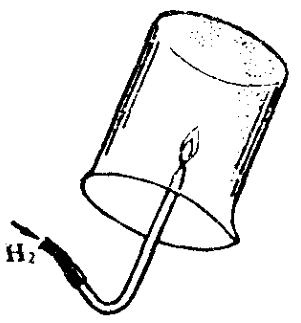
\includegraphics[width=4cm]{../pic/czhx1-xssy-21}
            \caption{氢气的可燃性}\label{fig:xssy-21}
        \end{minipage}
        \qquad
        \begin{minipage}[b]{7cm}
            \centering
            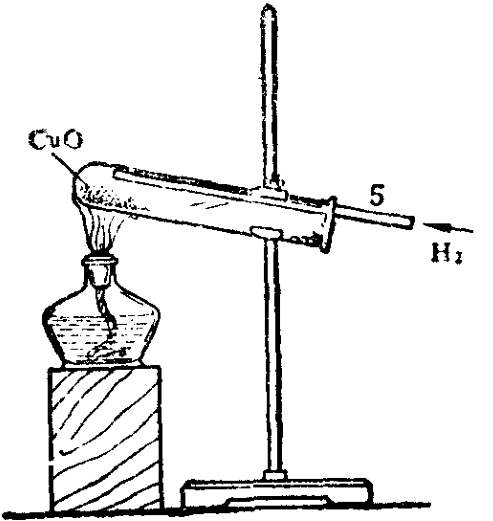
\includegraphics[width=6cm]{../pic/czhx1-xssy-22}
            \caption{氢气还原氧化铜}\label{fig:xssy-22}
        \end{minipage}
    \end{figure}

    (2) 氢气的还原性

    取少量氧化铜铺在干燥的试管的底部,按图 \ref{fig:xssy-22} 装置好。把导管 3 换成直导管 5。注意把试管口稍略微向下倾斜。
    通入经检验已证明是纯净的氢气,大约过一分钟,再加热试管里铺有氧化铜的部位。观察试管里发生的现象,写出这个反应的化学方程式。
\end{shiyanbuzhou}


\begin{wentihetaolun}
    1. 根据上面所做的实验,叙述氢气的物理性质和化学性质。

    2. 根据氢气的性质,可以采用哪些方法收集氢气?

    3. 点燃氢气前,为什么要检验氢气的纯度?怎样检验?

    4. 做氢气的还原性实验时,当氢气刚通入盛有氧化铜的试管时,能不能立即给试管加热?为什么?
\end{wentihetaolun}

